\documentclass[a4paper, titlepage]{report}

\usepackage[francais]{babel}
\usepackage[utf8]{inputenc}
\usepackage[T1]{fontenc}

\usepackage{listings}
\usepackage{titlesec}
\usepackage{color}
\usepackage{graphicx}

\titleformat{\chapter}[display]
  {\bfseries\Large}
  {\filright\textsc{\chaptertitlename} \LARGE\thechapter}
  {1ex}
  {\titlerule\vspace{1ex}\filleft}
  [\vspace{1ex}\titlerule]


\definecolor{gris}{rgb}{0.97,0.97,0.97}
\definecolor{vert}{rgb}{0,0.6,0}
\definecolor{mauve}{rgb}{0.5,0,0.5}
\definecolor{rose}{rgb}{1,0.5,1}
\definecolor{cyan}{rgb}{0.1,0.4,0.6}
\definecolor{marron}{rgb}{0.4,0.2,0}
\definecolor{jaune}{rgb}{1,0.6,0}
\definecolor{bleu}{rgb}{0,0,0.8}

\lstset{
	language=R,	
	frame=tblr,
	numbers=left,
	breaklines=true,
	backgroundcolor=\color{gris},
    basicstyle=\small\ttfamily,
    stringstyle=\color{vert},
    otherkeywords={0,1,2,3,4,5,6,7,8,9},
    morekeywords={TRUE,FALSE},
    deletekeywords={data,frame,length,as,character},
    keywordstyle=\color{blue},
    commentstyle=\color{vert},
}


\title{Rapport Projet SY09}
\date{3 mai 2018}
\author{Yiqing \textsc{Su} et Théophile \textsc{Molcard}}


\begin{document}

\renewcommand{\chaptername}{Partie}


\maketitle

\tableofcontents



\chapter{Cuisine}

Le jeu de données à étudier de la première partie est un ensemble de recettes de cuisine de diverses origines.\\
\indent Pour la question de 1.1 jusqu'à 1.5, le jeu de données utilisé est une version agrégée par origine. Puis pour les restes questions, il s'agit d'utiliser les données sans agrégation, autrement dit, il y a toutes les recettes de chaque pays ou région.

\section{Analyse exploratoire}
Le premier jeu de données comporte 26 lignes et 51 colonnes. Une ligne représente des informations synthétiques d'une recette pour un pays ou une région. Puis la première colonne indique le nom du pays ou de la région et les autres colonnes représentent l'utilisation des 50 ingrédients dans la recette. Les pays et les régions indiqués dans ces données sont asiatiques, européens ou américains.\\
\indent Avec \textbf{boxplot} et \textbf{summary}, nous pouvons voir que les données sont toutes entre 0 et 1. La moyenne pour chaque boîte à moustache est inférieur à 0,5. Parmi tous les pays ou régions, il y a plus que deux tiers qui ne sont pas asiatiques. Donc, les ingrédients comme "olive oil" et "cayenne" ont plus de variances parce que certains recettes utilisent beaucoup cet ingrédient et les autres non. Les ingrédients comme "soy sauce" et "sesame oil" sont faibles à la moyenne et à la variance parce que seulement les pays et les régions asiatiques vont les utiliser.\\
\indent Nous nous intéressons par la corrélation entre les données. Figure 1.1 et Figure 1.2 montrent la corrélation de manière que plus la couleur est foncé, plus la corrélation est forte. Dans Figure 1.1, nous pouvons voir qu'il y a beaucoup d'ingrédients corrélés entre eux et il y a une partie de corrélations fortes. Plus précisément, en calculant la proportion nous savons que les coefficients de corrélation qui sont plus que 0.3 ont pris une partie presque un moitié (47.2\%). Dans Figure 1.2, nous pouvons voir clairement qu'il existe beaucoup de relations entre les données. Il semble normal parce que nous avons vu que les recettes de pays viennent principalement la région asiatique, la région européenne et la région américaine.
\begin{figure}[htbp]
\centering
\begin{minipage}[t]{0.5\textwidth}
\centering
\includegraphics[width=6.5cm]{./doc/plot-correlation-cuisine1.png}
\caption{Corrélation entre les ingrédients}
\end{minipage}
\begin{minipage}[t]{0.48\textwidth}
\centering
\includegraphics[width=5cm]{./doc/plot-correlation-cuisine1_2.png}
\caption{Corrélation entre les recettes de pays}
\end{minipage}
\end{figure}


\section{Analyse en composantes principales}
La matrice que l'on étudie est de dimension $M_{26,50}$, elle est donc de rang inférieur à 26. L'inertie peut donc être entièrement expliquée par 26 composantes. En effectuant une ACP sur ces données on obtient donc les 26 composantes principales expliquant l'inertie du nuage de points. Si l'on cherche les valeurs propres de la matrice de covariance, on constate comme attendu que 24 des valeurs propres qui résultent sont nulles.\\

\newpage
On peut donc afficher l'inertie expliquée par chaque composantes et par la somme des n premiers axes.
\begin{figure}[h]
	\begin{center}
		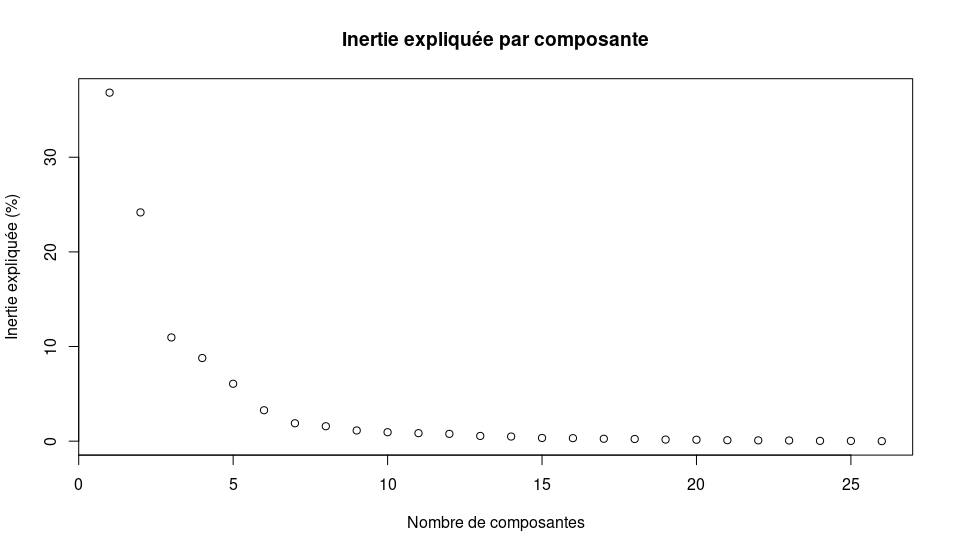
\includegraphics[scale = 0.32]{./doc/plot-inertie-par-composantes.png}
		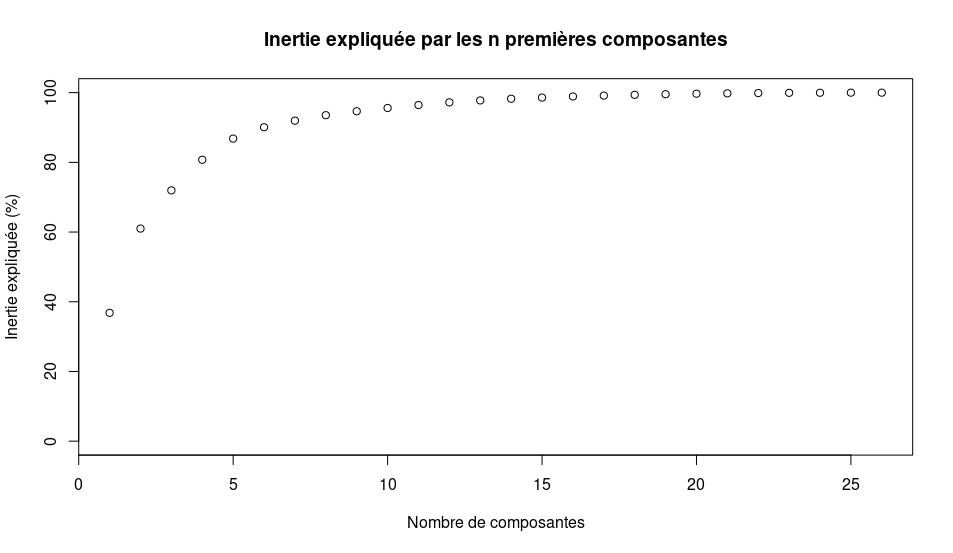
\includegraphics[scale = 0.32]{./doc/plot-inertie-n-composantes.png}
	\end{center}
\end{figure}

On constate que les deux premières composantes, bien qu'insuffisantes pour expliquer complètement les différences entre tous les points, permettent d'expliquer plus de 60\% de l'inertie. Il peut donc être intéressant d'afficher les points en fonction de ces composantes.
\begin{figure}[h]
	\begin{center}
		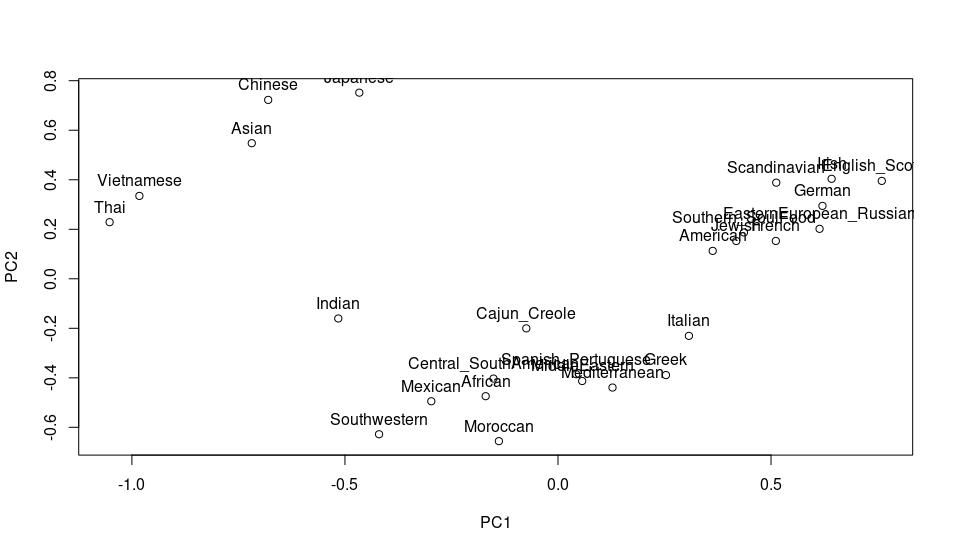
\includegraphics[scale = 0.32]{./doc/plot-recettes-composantes-1-2.png}
	\end{center}
\end{figure}

Par ce simple graphique on constate déjà certains regroupement entre les recettes des différents pays, avec trois groupes principaux qui ressortent. grossièrement on a les recettes des pays asiatiques, des pays occidentaux et des pays méditerranéens. Ces deux composantes sont cependant insuffisantes à expliquer l'ensemble des subtilités de ces données, 6 composantes sont nécessaire pour expliquer 90\% de l'inertie.

On peut par exemple être surpris par la proximité entre les recettes des pays d’Amérique centrale et méditerranéens ou africains. En effet cette proximité disparaît si l'on affiche cette fois les points suivant les composante 1 et 3.
\begin{figure}[h]
	\begin{center}
		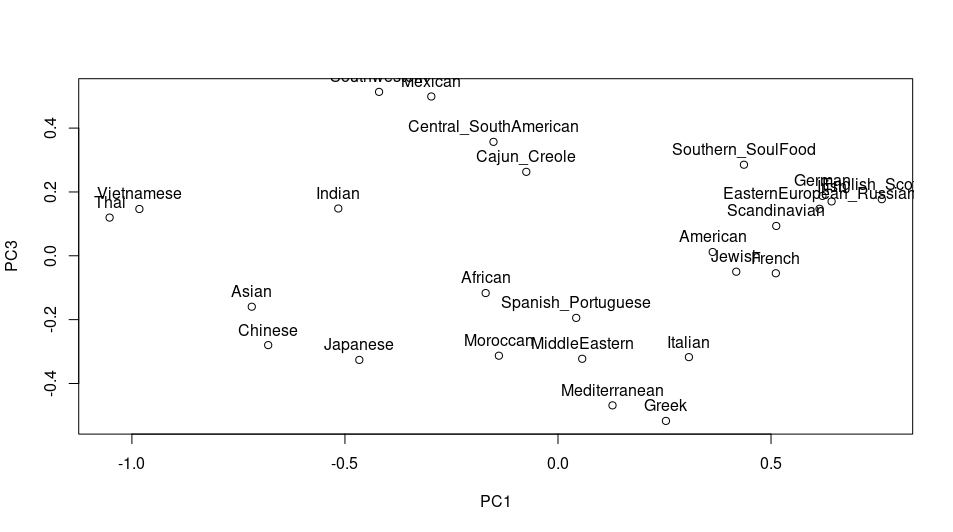
\includegraphics[scale = 0.32]{./doc/plot-recettes-composantes-1-3.png}
	\end{center}
\end{figure}

\section{Analyse ascendante hiérarchique}
Nous avons choisi la méthode de Ward. Le critère de Ward est un critère d'inertie qui représente l'inertie inter-classe de deux classes quand nous faisons une fusion entre ces deux classes, donc en minimisant ce critère, nous pouvons obtenir une optimisation locale. En addition, les résultats obtenu par le critère d'inertie sont conjointement à la méthode ACP.
\begin{figure}[h]
	\begin{center}
		\includegraphics[scale = 0.32]{./doc/plot-CAH.png}
	\end{center}
\end{figure}

\section{K-Means}

En premier lieu on utilise une méthode du coude pour déterminer combien de centres il serait judicieux de choisir.

\begin{figure}[h]
	\begin{center}
		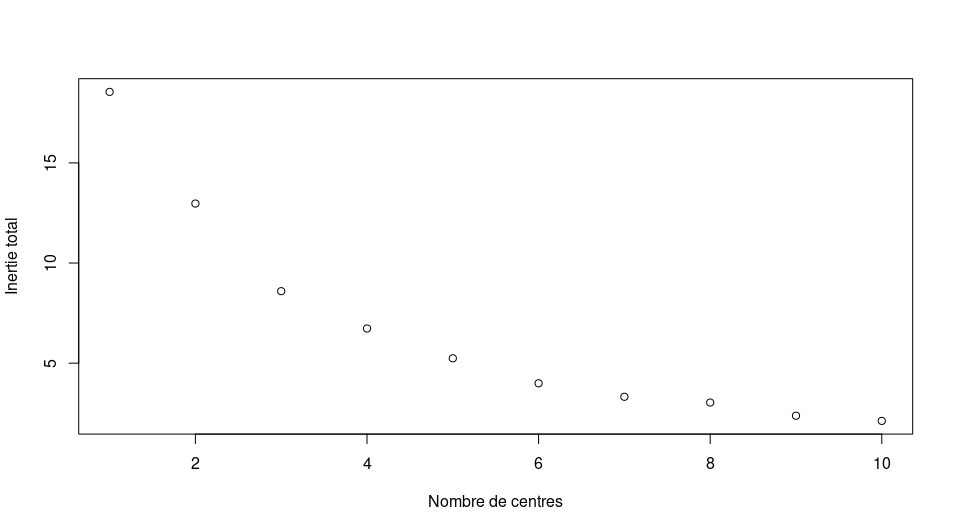
\includegraphics[scale = 0.32]{./doc/plot-kmeans-mininertie.png}
	\end{center}
\end{figure}

Ce graphe ne révèle pas de manière très net le nombre de groupes à sélectionner, on constate quand même qu'il y a une certaine rupture quand on dépasse les 3 groupes, et une autre moins évidente au delà de 5 groupes. 

\begin{figure}[h]
	\begin{center}
		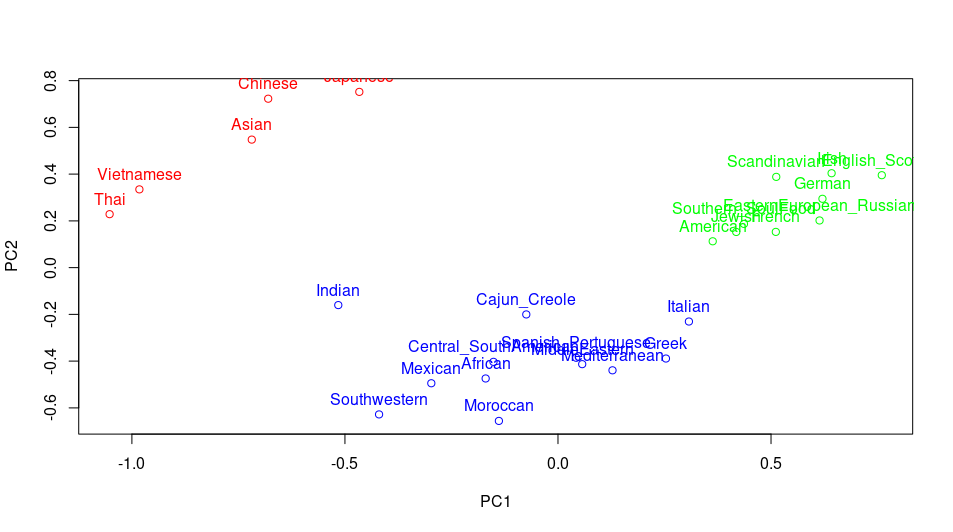
\includegraphics[scale = 0.32]{./doc/plot-kmeans-3.png}
	\end{center}
\end{figure}

En utilisant 3 groupes, on retrouve les groupes qui semblaient se dégager lors de l'ACP en affichant les points sur les deux composantes principales. 

\begin{figure}[h]
	\begin{center}
		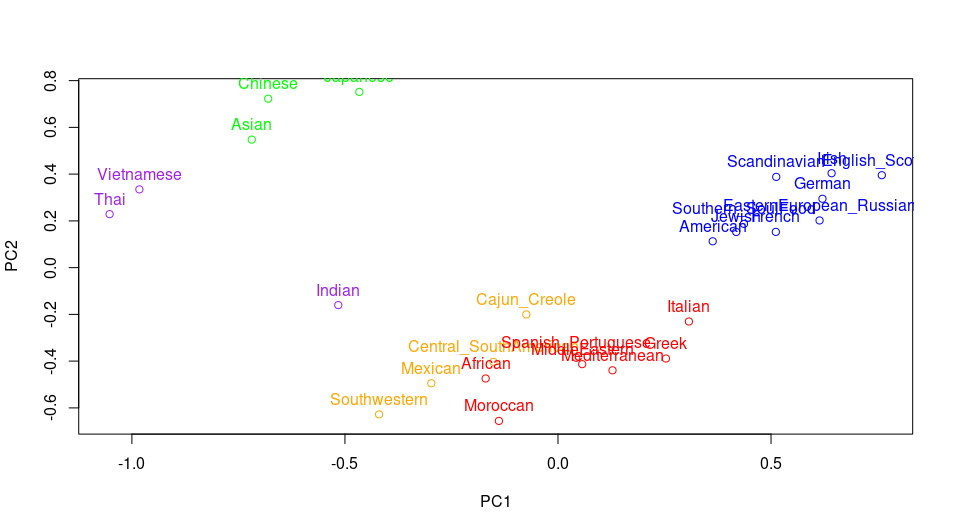
\includegraphics[scale = 0.32]{./doc/plot-kmeans-5.png}
	\end{center}
\end{figure}

La division en 5 groupes révèle une nouvelle division intéressante en séparant cette fois la cuisine des pays d’Amérique centrale des pays méditerranéens. Et en divisant les cuisines des pays asiatiques en deux groupes distincts.


\section{Comparaison}

On remarque très nettement, que ce soit en observant les données par rapport aux composantes principales obtenues avec l'ACP, à partir de l'analyse ascendante hiérarchique ou encore par l'algorithme des K-Means que les données semblent se regrouper en fonction de la situations géographique des pays étudiés. Cela semble tout à fait cohérent et c'est ce à quoi on pouvait s'attendre.
Les plats des différents pays sont généralement basés sur les aliments locaux, et plus des pays sont proches plus ces aliments seront susceptibles d'être similaires. Ainsi des traditions culinaires se sont développées sur la base de ces ingrédients, c'est pourquoi il est plus fréquent de trouver de la sauce soja dans les plats chinois et japonais que dans les plats français et allemands et et inversement pour le blé.
De plus les recettes sont issues des traditions culinaires et culturelle, qui sont également influencées par la proximité territoriale des régions. Que ce soit par le commerce ou par un mélange de cultures cela a également un impact sur l'alimentation d'une population. Cette aspect culturel de la cuisine explique également la forte similarité observable entre les recettes de pays pourtant très éloignées. On peut citer l'Amérique du Nord, malgré sa distance de l'Europe, les recettes apparaissent ici très similaires. On peut associer ça à sa colonisation par l'Europe qui y a imposé sa culture.


\section{Analyse descriptive}

- 2000 recettes
- 50 ingredients / 26 pays différents
- répartition des recettes inégale

\begin{figure}[h]
	\begin{center}
		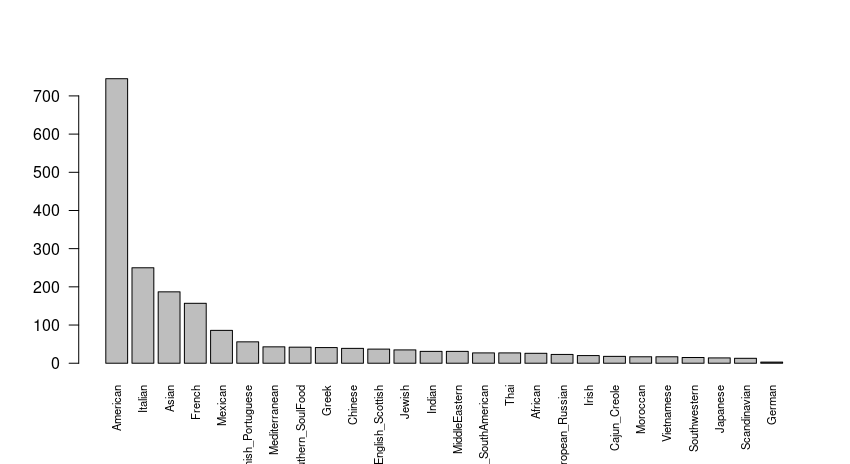
\includegraphics[scale = 0.32]{./doc/nombre-recettes.png}
	\end{center}
\end{figure}

1 = present dans une recette 
0 = absent

\section{Similarité - Dissimilarités}

Pour transformer ce tableau en tableau individu variables portant sur les ingrédients il semble intéressant de calculer une fréquence d'apparition d'un ingrédient sur toutes les recettes d'un pays. Cela revient à faire la moyenne de toutes les valeurs de chaque ingrédient pour un même pays. Ainsi, même si un type de cuisine est moins représenté que les autres, les aliments de base de cette cuisine apparaîtront avec de forts coefficients dans la colonne représentant le pays en question.
Cela permet de palier à la répartition très inégale des origines des recettes que l'on a a disposition.

On choisit la distance euclidienne psk fuck yeah !


\section{Classification ascendante hiérarchique}

\section{K-Médïodes}



\chapter{K-Means Adaptatif}


\section{Données synthétiques}

\section{Iris}

\section{Spam}



\chapter*{Annexe}
\lstinputlisting[firstline=0, lastline=108]{./doc/partie-1.R}


\end{document}
